\documentclass[Royal,times,sageh]{sagej}

\usepackage{moreverb,url,natbib, multirow, tabularx}
\usepackage[colorlinks,bookmarksopen,bookmarksnumbered,citecolor=red,urlcolor=red]{hyperref}





\begin{document}

\title{Missing the Point: Non-Convergence in Iterative Imputation Algorithms}

\runninghead{Oberman}

\author{H. I. Oberman\affilnum{1}}

\affiliation{\affilnum{1}{Department of Methodology and Statistics, Utrecht University, Utrecht,
The Netherlands}}

\corrauth{Hanne Oberman, Sjoerd Groenman building, Utrecht Science Park, Utrecht,
The Netherlands.}

\email{\href{mailto:h.i.oberman@uu.nl}{\nolinkurl{h.i.oberman@uu.nl}}}

\begin{abstract}
Iterative imputation is a popular tool to accommodate missing data.
While it is widely accepted that valid inferences can be obtained with
this technique, these inferences all rely on algorithmic convergence.
There is no consensus on how to evaluate the convergence properties of
the method. This paper provides insight into identifying non-convergence
of iterative impuation algorithms.
\end{abstract}

\keywords{missing data, iterative imputation, non-convergence, mice}

\maketitle

\hypertarget{introduction}{%
\section{Introduction}\label{introduction}}

Anyone who analyzes person-data may run into a missing data problem.
Missing data is not only ubiquitous, but treating it can also be
tedious. If a dataset contains just one incomplete observation,
statistical inferences are undefined and will not produce any results.
To circumvent this, many statistical packages employ list-wise deletion
by default (i.e., ignoring incomplete observations). Unfortunately, this
\emph{ad hoc} solution may yield wildly invalid results \citep{buur18}.
An alternative is to \emph{impute} (i.e., fill in) the missing values in
the incomplete observations. Subsequently, statistical inferences can be
performed on the completed dataset. By repeating this process several
times, a distribution of plausible results may be obtained, which
reflects the uncertainty in the data due to missingness. This technique
is known as `multiple imputation' \citep[MI;][]{rubin76}. MI has proven
to be a powerful technique to yield unbiased and confidence valid
estimates of the true---but missing---data inference under many
circumstances \citep{buur18}.

Figure \ref{fig:diagram} provides an overview of the steps involved with
MI---from incomplete data, to \(M\) multiply imputed datasets, to \(M\)
estimated quantities of interest \(\hat{Q}\)s, to a single pooled
estimate \(\bar{Q}\). Missing data in dataset \(y\) is imputed \(M\)
times. The imputed data \(y_{imp}\) is combined with the observed data
\(y_{obs}\) to create \(M\) completed datasets. On each completed
dataset, the analysis of scientific interest is performed. The quantity
of scientific interest (e.g., a regression coefficient) is denoted with
\(Q\). Since \(Q\) is estimated on each completed dataset, \(M\)
separate \(\hat{Q}\)-values are obtained. These \(M\) values are
combined into a single pooled estimate \(\bar{Q}\).

\begin{figure}

{\centering 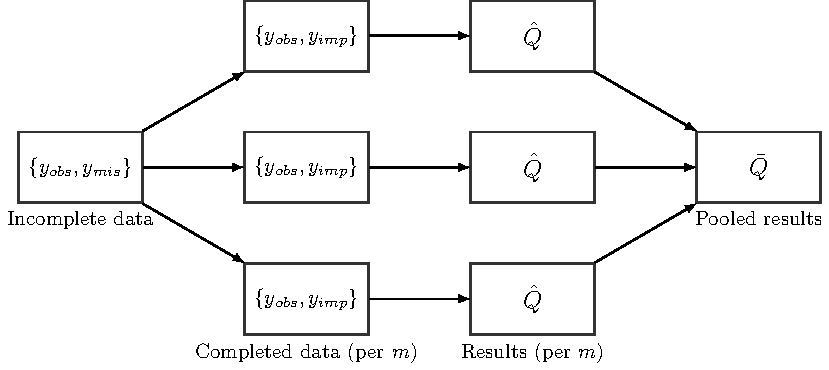
\includegraphics[width=\linewidth]{./images/diagram} 

}

\caption{Scheme of the main steps in multiple imputation.}\label{fig:diagram}
\end{figure}

A popular method to obtain imputations is to use the `Multiple
Imputation by Chained Equations' algorithm, shorthand
`MICE'\citep{mice}. MICE is an iterative algorithmic procedure to draw
imputations from the posterior predictive distribution of the missing
values. This introduces a potential threat to the validity of the
imputations: What if the algorithm has not converged? Are the
implications then to be trusted? And can we rely on the inference
obtained on the completed data? These are all open questions, because
the convergence properties of iterative imputation algorithms have not
been systematically studied \citep{buur18}. Moreover, there is no
scientific consensus on how to evaluate convergence of MI algorithms
\citep{taka17}. Some default MICE techniques (e.g., `predictive mean
modeling') might not yield converged states at all \citep{murr18}.
Therefore, algorithmic convergence should be monitored carefully.

Currently, the recommended practice for evaluating convergence in
iterative imputation algorithms is to visually inspect imputations for
signs of non-convergence. \textbf{Add that this refers to chain means
and variances already? It's insufficient that these are univariate, so
multivariate state space of the algorithm may not be converged when
univariates are ok. And \citet{buur18}`s suggestion to track
user-defined statistics (e.g., regression coefficient) may be somewhat
advanced for empirical researchers. Moreover, this is not
model-independent, i.e., only apply to one substantive model, while one
of the advantages of MI is that missing data problem and scientific
problem are split. Then we can say 'we propose a novel\ldots{}' and
integrate this: Note that usually we only evaluate the convergence of
univariate scalar summaries (e.g., chain means or variances). With these
we cannot diagnose convergence of multivariable statistics (i.e.,
relations between scalar summaries). Van Buuren \citeyearpar[\(\S\)
4.5.2]{buur18} proposed to implement multivariable evaluation of the
MICE algorithm through eigenvalue decomposition building on the work of
\citet{mack03}. Eigenvalues of a covariance matrix are a measure of the
data's covariance.}.

This method is insufficient on two counts: 1) it may be challenging to
the untrained eye, and 2) only severely pathological cases of
non-convergence may be diagnosed \citep[\(\S\) 6.5.2]{buur18}.
Therefore, a quantitative, diagnostic evaluation of convergence would be
preferred. Yet, monitoring convergence of iterative imputation
algorithms diagnostically is challenging. Iterative imputation
algorithms such as MICE are Markov chain Monte Carlo (MCMC) methods. In
MCMC methods, convergence is not from a scalar to a point but from one
distribution to another. The values generated by the algorithm (e.g.,
imputed values) will vary even after convergence. Therefore, the aim of
convergence diagnostics for MCMC methods is not to establish the point
at which convergence is reached, but to monitor signs of non-convergence
\citep{hoff09}. Several of such diagnostics exist for MCMC methods, but
it is not known whether these are appropriate for iterative imputation
algorithms.

In this paper, we investigate how non-convergence in iterative
imputation algorithms may be diagnosed, how well these methods perform,
and at which point convergence may safely be assumed. For reasons of
brevity, we only focus on the iterative imputation algorithm implemented
in the popular \texttt{mice} package \citep{mice} in \texttt{R}
\citep{R}. The convergence properties of the MICE algorithm are
investigated through model-based simulation. The results of this
simulation study are guidelines for assessing convergence of MI
algorithms, which will aid applied researchers in drawing valid
inference from incomplete datasets.

\textbf{Include sub-questions!} How can non-convergence be identified
diagnostically? Are common MCMC non-convergence diagnostics appropriate
for MICE? And if so, which threshold should be used to diagnose
non-convergence? How many iterations are sufficient/needed to be able to
diagnose non-convergence? Are the default number of iterations
sufficient (i.e., 5 in mice, 10 in SPSS and Stata, 30 in mi)?
\textbf{How severe is it when the algorithm has not converged? And what
are guidelines for practice? Can the parameter of interest, estimand
\(Q\), be correct when the algorithm is not (yet) converged, and vice
versa?} \emph{(Maybe add these too? What are the effects of continued
iterations on estimates, predictions and inferences? Do the answers
differ with varying missingness proportions? That is, we vary the nr of
iterations and the missingness proportion because we assume that the
algorithm has not reached convergence at \(t=1\), and performs worse
with moderate to high missingness (not so much with little or a LOT of
missingness).)}

\hypertarget{some-notation}{%
\subsection{Some notation}\label{some-notation}}

Let \(y\) denote an \(n \times k\) matrix containing the data values on
\(k\) variables for all \(n\) units in a sample. The data value of unit
\(i\) (\(i = 1, 2, \dots, n\)) on variable \(j\)
(\(j = 1, 2, \dots, k\)) may be either observed or missing. \textbf{The
number of units \(i\) with at least one missing data value can be
divided by the total number of units \(n\) to obtain the `missingness
proportion' \(p_{mis}\).} The collection of observed data values in
\(y\) is denoted by \(y_{obs}\); the missing part of \(y\) is referred
to as \(y_{mis}\). For each datapoint in \(y_{mis}\), we sample
\(M \times T\) times plausible values, where \(M\) is the number of
imputations (\(m = 1, 2, \dots, M\)) and \(T\) is the number of
iterations (\(t = 1, 2, \dots, T\)). The collection of samples between
the initial value (at \(t=1\)) and the final imputed value (at \(t=T\))
will be referred to as an `imputation chain'. \textbf{Add: \(\theta\)s
are scalar summaries of interest in the iterative algorithm (e.g., chain
means; the average of the imputed values in each imputation chain). }

\hypertarget{identifying-non-convergence}{%
\section{Identifying
non-convergence}\label{identifying-non-convergence}}

The goal of imputation through e.g.~FCS/MICE is to pbtain a multivariate
distribution by iterating over the sequence of univariate imputations.
Traditionally, the inspection of the multivariate convergence is done by
visually inspecting the univariate chain means and variances over the
iterations, or by tracking the Rhat and autocorrelation. The downside to
these approaches is that they either focus on the univariate state
space, or primarily track the change over the iterations of a
multivariate outcome conform the scientific model of interest. Focusing
on the convergence of these outcome parameters may influence this
procedure in the sense that the model of evaluation favors the model of
interest. Ideally, one would like to evaluate a model-independent
parameter that summarizes the multivariate nature of the data. We
propose eigenvalue as such a parameter, because it\ldots.

Mixing and stationarity have histroically been inspected visually, by
evaluating traceplots of scalar summaries of interest (\(\theta\)s;
e.g., chain means and chain variances). As \citet{buur18} describes,
users can also specify a model-specific scalar summary (e.g., a
regression coefficient). A user-specified scalar summary, however, is
not universal to all complete data problems. Therefore, as inspired by
\citep{mack03}, we propose a \(\theta\) that summarizes the multivariate
state space of the algorithm. Namely, the first eigenvalue of the
variance-covariance matrix of the \(M\) completed datasets. \textbf{The
first eigenvalue has the appealing property that is not dependent on the
substantive model of interest.}

\textbf{Since convergence of iterative imputation algorithms is in
distribution, there is not a unique point at which the algorithm reaches
a converged state. We can only evaluate scalar summaries of the
multivariate state space of the algorithm, \(\theta\)s. The recommended
scalar summaries to evaluate are chain means and chain variances.
Additionally, researchers may ``monitor some statistic of scientific
interest'' \citep[\(\S\) 6.5.2]{buur18}. Because of the issues mentioned
above, we propose a novel \(\theta\) to monitor: the first eigenvalue of
the variance-covariance matrix of the completed data. Let
\(\lambda_1 \geq \lambda_2 \geq ... \geq \lambda_j\) be the eigenvalues
of \(\Sigma\) in each of the \(M\) completed datasets
\({y_{obs}, y_{imp}}\). \(\lambda_1\) is measure that summarises the
covariances in the completed datasets.}

There are two requirements for convergence of iterative algorithms:
mixing and stationarity \citep{gelm13}. Without mixing, imputation
chains do not intermingle nicely, \textbf{indicating that \ldots{}}.
Without stationarity, there is trending within imputation chains, which
implies that further iterations would yiled a different set of
imputations.

To illustrate what non-convergence looks like in MI, we reproduce the
example from van Buuren \citeyearpar[\(\S\) 6.5.2]{buur18}. Figure
\ref{fig:non-conv} shows the traceplot for one of the variables in the
example. we see the average of the imputed values for a variable \(j\)
in \(y_{imp}\). The average imputed values in the left hand plot are
about a magnitude 2 lower than the right hand plot. So non-convergence
has a impact on the average imputed value for \(j\) in \(y_{imp, m}\).
This difference (presumably) translates to bias in the pooled estimate
\(\bar{\mu}_j\) as well. And maybe also to higher order statistics,
e.g.~variances, covariances, etc. Therefore, it's important to converge.
\textbf{Explain what we see, namely example by \citet{buur18}
reproduced, showing the traceplots of chain means for some variable. The
first plot is typical convergence of MICE, the second is pathological
non-convergence because of a mis-specified imputation model. Each line
is an imputation. In the first plot, the chains intermingle nicely and
there is little to no trending. In the second plot, there is a lot of
trending and some chains do not intermingle. Importantly, the chain
means at the last iteration (the imputed value per \(m\)) are very
different between the two plots. The algorithm with the mis-specified
model yields imputed values that are on average a magnitude two larger
than those of the typically converged algorithm. This shows the
importance of reaching converged states in iterative imputation
algorithms.}

\hypertarget{methods-under-evaluation}{%
\subsection{Methods under evaluation}\label{methods-under-evaluation}}

Non-stationarity within chains may be diagnosed with e.g.,
autocorrelation \citep[\(AC\);][]{scha97, gelm13}, numeric standard
error \citep[`MC error';][]{gewe92}, or Raftery and Lewis's
\citeyearpar{raft91} procedure to determine the effect of trending on
the precision of estimates. A widely used diagnostic to monitor mixing
between chains is the potential scale reduction factor \(\widehat{R}\)
\citep[`Gelman-Rubin statistic';][]{gelm92}. With a recently proposed
adaptation, \(\widehat{R}\) might also serve to diagnose
non-stationarity, but this has not yet been thoroughly investigated
\citep{veht19}. Therefore, use we \(\widehat{R}\) and \(AC\) to evaluate
mixing and stationarity separately, as recommended by e.g.,
\citet{cowl96}.

\begin{figure}

{\centering 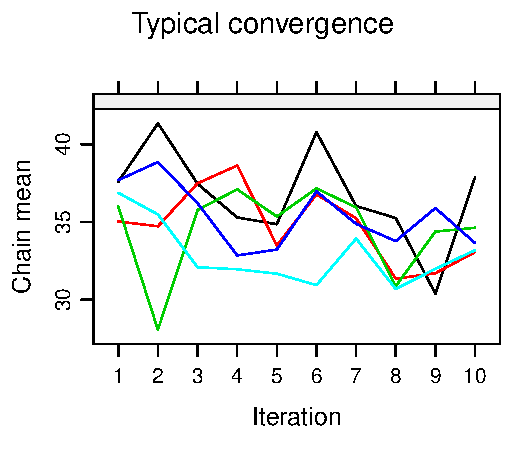
\includegraphics[width=.49\linewidth]{manuscript_files/figure-latex/non-conv-1} 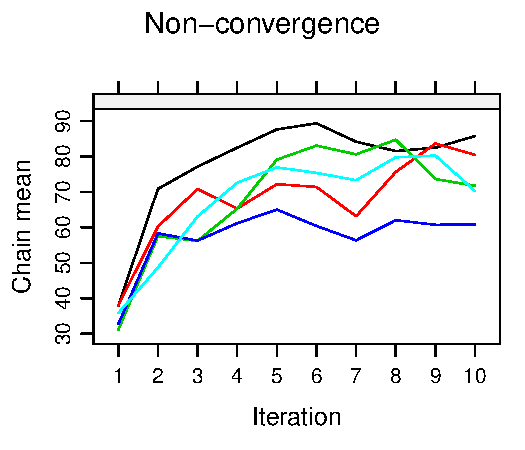
\includegraphics[width=.49\linewidth]{manuscript_files/figure-latex/non-conv-2} 

}

\caption{Typical convergence versus pathological non-convergence. Please note that this is the same data with a different imputation model, leading to different imputations (see the y axis!). Wel min of meer dezelfde origin op iteration 1.}\label{fig:non-conv}
\end{figure}

\hypertarget{potential-scale-reduction-factor}{%
\subsubsection{Potential scale reduction
factor}\label{potential-scale-reduction-factor}}

An updated version of \(\widehat{R}\) has been proposed by
\citet{veht19} (p.~5). \textbf{This version may be suitable for
iterative imputation.} Let \(M\) be the total number of chains, \(T\)
the number of iterations per chain, and \(\theta\) the scalar summary of
interest (e.g., chain mean or chain variance). For each chain
(\(m = 1, 2, \dots, M\)), we estimate the variance of \(\theta\), and
average these to obtain within-chain variance \(W\).

\begin{align*}
W&=\frac{1}{M} \sum_{m=1}^{M} s_{j}^{2}, \text { where } s_{m}^{2}=\frac{1}{T-1} \sum_{t=1}^{T}\left(\theta^{(t m)}-\bar{\theta}^{(\cdot m)}\right)^{2}. 
\end{align*}

We then estimate between-chain variance \(B\) as the variance of the
collection of average \(\theta\) per chain.

\begin{align*}
B&=\frac{T}{M-1} \sum_{m=1}^{M}\left(\bar{\theta}^{(\cdot m)}-\bar{\theta}^{(\cdot \cdot)}\right)^{2}, \text { where } \bar{\theta}^{(\cdot m)}=\frac{1}{T} \sum_{t=1}^{T} \theta^{(t m)} \text{, } \bar{\theta}^{(\cdot \cdot)}=\frac{1}{M} \sum_{m=1}^{M} \bar{\theta}^{(\cdot m)}. 
\end{align*}

From the between- and within-chain variances we compute a weighted
average, \(\widehat{\operatorname{var}}^{+}\), which over-estimates the
total variance of \(\theta\) \textbf{remove or explain why, or leave
in}. \(\widehat{R}\) is then obtained as a ratio between the
over-estimated total variance and the within-chain variance:

\begin{equation*}
\widehat{R}=\sqrt{\frac{\widehat{\operatorname{var}}^{+}(\theta | y)}{W}},
\text{ where } \widehat{\operatorname{var}}^{+}(\theta | y)=\frac{N-1}{N} W+\frac{1}{N} B.
\end{equation*}

We can interpret \(\widehat{R}\) as potential scale reduction factor
since it indicates by how much the variance of \(\theta\) could be
shrunken down if an infinite number of iterations per chain would be run
\citep{gelm92}. This interpretation assumes that chains are
`over-dispersed' at \(t=1\), and reach convergence as \(T \to \infty\).
Over-dispersion implies that the initial values of the chains are `far
away' from the target distribution and each other. When all chains
sample independent of their initial values, the mixing component of
convergence is satisfied, and \(\widehat{R}\)-values will be close to
one. High \(\widehat{R}\)-values thus indicate non-convergence. The
conventionally acceptable threshold for convergence was
\(\widehat{R} < 1.2\) \citep{gelm92}. More recently, \citet{veht19}
proposed a more stringent threshold of \(\widehat{R} < 1.01\).

\hypertarget{autocorrelation}{%
\subsubsection{Autocorrelation}\label{autocorrelation}}

Following the same notation, we define autocorrelation as the
correlation between two subsequent \(\theta\)-values within the same
chain \citep[p.~147]{lync07}. In this study, we only consider \(AC\) at
lag 1, i.e., the correlation between the \(t^{th}\) and \(t+1^{th}\)
iteration of the same chain.

\begin{equation*}
AC = \left( \frac{T}{T-1} \right) \frac{\sum_{t=1}^{T-1}(\theta_t - \bar{\theta}^{(\cdot m)})(\theta_{t+1} - \bar{\theta}^{(\cdot m)})}{\sum_{t=1}^{T}(\theta_t - \bar{\theta}^{(\cdot m)})^2}.
\end{equation*}

We can interpret \(AC\)-values as a measure of stationarity. If
\(AC\)-values are close to zero, there is no dependence between
subsequent samples within imputation chains. Negative \(AC\)-values
indicate divergence within imputation chains. \textbf{Subsequent sampled
values within each imputation chain are less alike.} Positive
\(AC\)-values indicate recurrence. If \(\theta\)-values of subsequent
iterations are similar, trending may occur. Negative \(AC\)-values show
no threat to the stationarity component of convergence. On the contrary
even---negative \(AC\)-values indicate that \(\theta\)-values of
subsequent iterations diverge from one another, which may increase the
variance of \(\theta\) and speed up convergence. As convergence
diagnostic, the interest is therefore in positive \(AC\)-values.
\textbf{Maybe remove:} Moreover, the magnitude of \(AC\)-values may be
evaluated statistically, but that is outside of our scope.

\hypertarget{in-practice}{%
\subsection{In practice}\label{in-practice}}

Upon convergence, \(\widehat{R}=1\) and \(AC=0\), which are unlikely
thresholds for MCMC algorithms, because of its convergence to a
distribution. In practice, non-convergence is usually diagnosed when
\(\widehat{R}\) \textgreater{} 1.2 or 1.1 or even 1.01. And a t-test is
performed to assess whether \(AC\) is significantly different from zero.

We assume that complete convergence, defined as \(\widehat{R} = 1\) and
\(AC = 0\), will not be observed. Because even in the most converged
state, the algorithm will show some signs of non-mixing and
non-stationarity. Upon \emph{sufficient} convergence, the imputation
chains will intermingle such that the only difference between the chains
is caused by the randomness induced by the algorithm
(\(\widehat{R} > 1\)), and there may be some dependency between
subsequent iterations of imputation chains (\(AC > 0\)).

\textbf{Before using them in the simulation, the two methods show at
least be able to distinguish between the two algorithms plotted in
Figure 2. From visual inspection we know that the typical convergence
has some signs of non-mixing around iteration 2, and little trending. In
the non-convergence situation, there is a lot of trending upto iteration
6, after which the chains reach a somewhat more stationary state. Mixing
in this situation gets worse from the first iteration onward, and
gradually gets better around iteration 7. To assess whether
\(\widehat{R}\) and \(AC\) may be appropriate non-convergence
identifiers for iterative imputation algorithms, the following condition
must hold: the methods indicate worse performance for the mis-specified
model with pathological non-convergence (i.e., higher \(\widehat{R}\)-
and \(AC\)-values than the typical performance). And additionally the
methods should reflect the increasing convergence in the typical
convergence situation as the number of iterations goes up.}

\textbf{In Figure \ref{fig:diagnostics}A, the chain means from Figure
\ref{fig:non-conv} are plotted again, now together---as are the
non-convergence diagnostics. Panel B shows \(\widehat{R}\) as computed
by implementing \citet{veht19} 's recommendations. As required,
\(\widehat{R}\) indicates less signs of non-convergence as the number of
iterations goes up }in the typical convergence situation\textbf{. The
superior performance of the typical convergence over the pathological
non-convergence is less prominent, even flipped for \(t<4\). Panel C
displays the \(AC\) as computed with the R function
\texttt{stats::acf()}. When we look at this panel, we conclude something
weird. The \(AC\)-values indicate equal performance (up-to \(t=5\)) for
the typical convergence and the pathological non-convergence, while
there is obvious trending in the latter. Moreover, the best convergence
(as indicated by the lowest \(AC\)-value) is observed at \(t=2\), but
looking at the chain means in panel A, there should be some signs of
trending up-to iteration number seven. After consulting the
documentation on stats::acf() \citep{R}, we conclude that this
implementation of \(AC\) is not suitable for iterative imputation
algorithms. There is a correction factor for a mathematical shortcut
that works in the limit. According to \citet{box15}, the function works
when the number of iterations \textgreater{} 50. The default number of
iterations in iterative imputation, however, is often much lower.
Therefore, we compute \(AC\) manually, see panel D. The AC values in
this plot do meet the requirements (\ldots) and will therefore be used
in the simulation study.}

\textbf{acf is niet bedoeld om weinig iteraties te\ldots{} niet een fout
in acf, alleen hier niet van toepassing}

\begin{figure}

{\centering 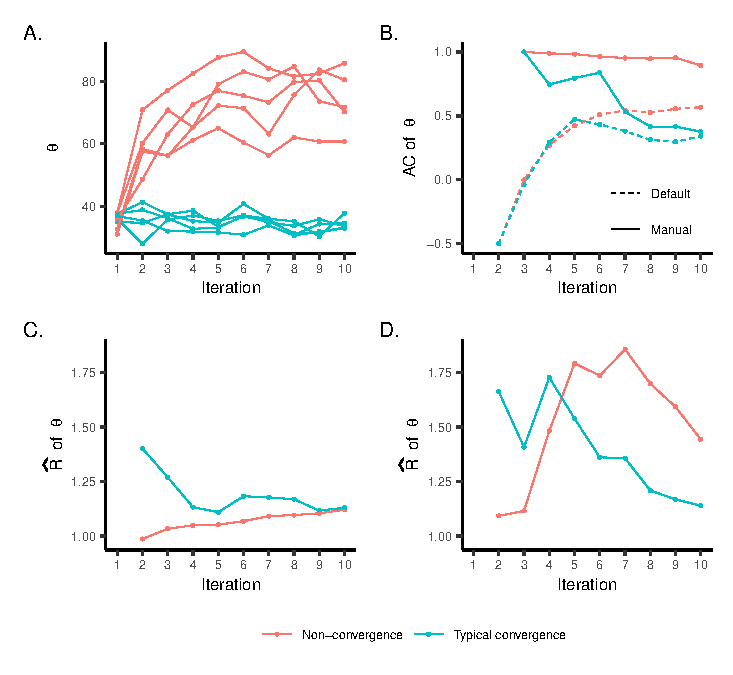
\includegraphics{manuscript_files/figure-latex/diagnostics-1} 

}

\caption{Convergence diagnostics applied on the imputation algorithms of Figure 2. $\theta$ = chain mean in $y_{imp, m}$.}\label{fig:diagnostics}
\end{figure}

\hypertarget{simulation-study}{%
\section{Simulation study}\label{simulation-study}}

The aim of the simulation study is to evaluate the impact of inducing
non-convergence in the MICE algorithm on several quantities of
scientific interest \(Q\). Subsequently we will evaluate how well
\(\widehat{R}\) and \(AC\) perform in identifying the effects of
non-convergence. And finally, we will formulate an informed advice on
the requirements to safely assume \emph{sufficient} convergence in
practice. That is, we assume that the algorithm is \emph{sufficiently}
converged when each estimate \(\bar{Q}\) is an unbiased and confidence
valid estimate of the corresponding estimand \(Q\).

Non-convergence will be induced by: 1) increasing the missingness
proportion \(p_{mis}\) in dataset \(y\) incrementally, and 2)
terminating the imputation algorithm at a varying number of iterations
\(T\). The first set of simulation conditions---the missingness
proportions---is chosen to reflect the difficulty of the missingness
problem. The underlying assumption is that low missingness proportions
lead to quick algorithmic convergence, since there is a lot of
information in the observed data. Higher missingness proportions should
yield slower convergence. Unless, however, the fraction of missing
information is so high that the random component in the imputation
algorithm outweighs the information in the observed data. Then,
convergence to a stable but highly variable state may be reached
instanteneously. We assume that the incremental missingness proportions
in our study will result in a corresponding increase in signs of
non-convergence.

The assumption inherent to the second set of simulation conditions---the
number of iterations---is that terminating the imputation algorithm too
early causes non-convergence. Generally, the algorithm will not reach
convergence if \(T=1\), because the imputed values in the first
iteration (at \(t=1\)) depend on the initial values of the algorithm
(which are sampled randomly from the set of observed datapoints). As the
number of iterations increases, the imputation chains should become
independent of the initial values, until the point at which adding an
extra iteration does not lead to a more converged state. We assume that
we can induce non-convergence at least in conditions where \(T\) is
smaller than the default number of iterations in \texttt{mice}, \(T=5\).

\hypertarget{hypotheses}{%
\subsection{Hypotheses}\label{hypotheses}}

\begin{enumerate}
\def\labelenumi{\arabic{enumi}.}
\item
  We expect that simulation conditions with a high missingness
  proportion \(p_{mis}\) and a low number of iterations \(T\) will
  result in biased, invalid estimates of the quantities of scientific
  interest, \(Q\)s.
\item
  We hypothesize that \(\widehat{R}\) and \(AC\) will correctly identify
  signs of non-convergence in those simulation conditions where the
  \(\bar{Q}\)s are \emph{not} unbiased and confidence valid estimates of
  the \(Q\)s.
\item
  We hypothesize that the recommended thresholds to diagnose
  non-convergence with \(\widehat{R}\) (\(\widehat{R} > 1.2\),
  \(\widehat{R} > 1.1\), and \(\widehat{R} > 1.01\)) may be too
  stringent for iterative imputation applications. In an empirical
  study, where \(\widehat{R}\) was used to inform the required
  imputation chain length, it took as many as 50 iterations to overcome
  the conventional non-convergence threshold \(\widehat{R}>1.2\). Yet,
  scientific estimates were insensitive to continued iteration after
  \(t>5\) \citep{lace07}. We therefore suspect that \(\widehat{R}\) may
  over-estimate signs of non-convergence in iterative imputation
  algorithms. In contrast to this, it may occur that the signs of
  non-convergence are under-estimated by \(\widehat{R}\), in exceptional
  cases where the initial values of the algorithm are not appropriately
  over-dispersed \citep[p.~437]{broo98}. In e.g.~\texttt{mice}, initial
  values are chosen randomly from the observed data, hence we cannot be
  certain of over-dispersion in the initial values. In practice, we do
  not expect this to cause problems for identifying non-convergence with
  \(\widehat{R}\).
\item
  We expect that high \(AC\) values are implausible in iterative
  imputation algorithms with typical convergence. That is, after only a
  few iterations, the randomness induced by the algorithm will
  effectively mitigate the risk of dependency within chains.
\end{enumerate}

\hypertarget{set-up}{%
\subsection{Set-up}\label{set-up}}

Convergence of the MICE algorithm is investigated through model-based
simulation in \texttt{R} \citep[version 3.6.3;][]{R}. The simulation
set-up is summarized in the pseudo-code below. The complete \texttt{R}
script of the simulation study is available from
\href{https://github.com/gerkovink/shinyMice/tree/master/3.Thesis/1.SimulationStudy}{github.com/gerkovink/shinyMice}.

\begin{verbatim}
# pseudo-code of simulation 
1. simulate data 
for (number of simulation runs from 1 to 1000)
 for (missingness proportions 5%, 25%, 50%, 75% and 95%)
  2. create missingness
  for (number of iterations from 1 to 100)
   3. impute missingness
   4. perform analysis of scientific interest
   5. compute non-convergence diagnostics 
   6. pool results across imputations
   7. compute performance measures
 8. combine outcomes of all missingness proportions
9. aggregate outcomes across simulation runs 
\end{verbatim}

\hypertarget{data-generating-mechanism.}{%
\subsubsection{Data-generating
mechanism.}\label{data-generating-mechanism.}}

In this study, sampling variance is not of interest. Therefore, a single
complete dataset may serve as comparative truth in all simulation
repetitions \citep{vink14}. The data-generating mechanism is a
multivariate normal distribution, representing person-data on three
predictor variables in a multiple linear regression problem
\textbf{(from an unspecified social scientific field of study)}. Let the
predictor space be defined as \[
\begin{aligned}
\begin{pmatrix}X_1\\
X_2\\
X_3
\end{pmatrix} \sim \mathcal{N}
\begin{bmatrix}
\begin{pmatrix}
12\\
3\\
0.5
\end{pmatrix}\!\!,
\begin{pmatrix}
4 & 4 & 1.8 & 0\\
4 & 16 & 4.8 & 0\\
1.8 & 4.8 & 9 & 0
\end{pmatrix}
\end{bmatrix}\!\!\text{.}\\[2\jot]
\end{aligned}
\] A finite population of \(N=1000\) is simulated using the
\texttt{mvtnorm} package \citep{mvtnorm}. Subsequently, a fourth
variable is constructed as outcome \(Y\). For each unit
\(i = 1, 2,..., N\), let \[
Y_i = 1 + 2X_{1i} +.5X_{2i} - X_{3i} + \epsilon_i ,
\] where \(\epsilon \sim \mathcal{N}(0, 100)\). From the complete set,
we obtain the true values of each quantity of scientific interest \(Q\).

\hypertarget{scientific-estimands.}{%
\subsubsection{Scientific estimands.}\label{scientific-estimands.}}

We consider four types of \(Q\)s that are often of interest in empirical
research. Namely, two descriptive statistics: the mean \(\mu_j\) and
standard deviation \(\sigma_j\) of each variable
\(j = Y, X_1, X_2, X_3\). We also consider the regression coefficients
of the predictors: \(\beta_1\), \(\beta_2\), and \(\beta_3\) in
regression equation
\[Y' = \beta_0 + \beta_1 X_1 + \beta_2 X_2 + \beta_3 X_3,\] where \(Y'\)
is the expected value of the outcome. And finally, the proportion of
variance explained by the set of predictors: coefficient of
determination \(r^2 \times 100\) \textbf{(note that lower case \(r\) is
used to avoid confusion with non-convergence diagnostic
\(\widehat{R}\))}. The true values of these scientific estimands are
calculated with the R functions \texttt{base::mean()},
\texttt{stats::sd()}, and \texttt{stats::lm()} \citep{R}. Each of these
\(Q\)s is estimated with a corresponding \(\bar{Q}\), after the complete
dataset is first \emph{amputed} (with a varying missingness proportion
\(p_{mis}\)) and subsequently imputed (with a varying number of
iterations \(T\)).

\hypertarget{methods.}{%
\subsubsection{Methods.}\label{methods.}}

The complete dataset is amputed with the \texttt{mice} package
\citep[function \texttt{mice::ampute()};][]{mice}. All missingness is
multivariate, and conform a `missing completely at random' missingness
mechanism \citep{rubin87}. I.e., the probability to be missing is the
same for all \(N \times k\) cells in \(y\), conditional on the
missingness proportion (\(p_{mis} =.05,.25,.5,.75,.95\)).

Missing datapoints in \(y\) are imputed with the \texttt{mice()}
function \citep{mice}. All imputation procedures are performed with
Bayesian linear regression imputation, and five imputation chains
(\(M=5\)). The number of iterations varies between simulation conditions
(\(T=1,2,...,100\)).

After each run of the \texttt{mice} algorithm, the function
\texttt{mice::complete()} is used to combine the imputed data
\(y_{imp,m}\) with the observed data \(y_{obs}\), resulting in five
completed datasets \{\(y_{obs}, y_{imp, m}\)\}, where
\(m = 1, 2, ..., 5\).

\begin{itemize}
\item
  on the 5 imputations \(y_{imp,m}\): get mean and var within imp chains
  as theta to compute conv diag --\textgreater{} then complete with
  \texttt{mice::complete()}
\item
  on the 5 completed datasets \{\(y_{obs}, y_{imp, m}\)\}: 1) estimate
  Qhats for mu and sigma --\textgreater{} pool as mean()
  --\textgreater{} get Qbars of mu and sigma; 2) compute lambda as theta
  for conv diag; 3) perform lm to get Qhats for betas and r\^{}2
  --\textgreater{} use Qhats of beta as theta to compute conv diag
  --\textgreater{} pool Qhats of beta and r\^{}2 to get Qbars
\end{itemize}

The estimator for each \(Q\) is \(\bar{Q}\)---the pooled aggregate of
the \(\hat{Q}\)s across imputations. To calculate the \(\bar{Q}\)s, we
combine the observed data \(y_{obs}\) and the imputed data for each
imputation \(y_{imp,m}\) with the function \texttt{mice::complete()}.
Descriptive statistics are computed as the average across imputations
for each variable (\(\mu_j\) and \(\sigma_j\), where
\(j = Y, X_1, X_2, X_3\)). Estimated regression coefficients are
obtained with the function \texttt{stats::lm()} for each imputation, and
then pooled conform \citet{vink14}. The coefficient of determination is
estimated for each imputation, and pooled using
\texttt{mice::pool.r.squared()}.

For each run of the imputation algorithm, we compute non-convergence
diagnostics \(\widehat{R}\) and \(AC\). We calculate \(\widehat{R}\) by
implementing Vehtari et al.'s \citeyearpar{veht19} recommendations, and
\(AC\) as the correlation between the \(t^{th}\) and the \((t+1)^{th}\)
iteration. The two methods are applied to four scalar summaries
\(\theta\): chain means (i.e., the mean in each \(y_{imp, m, j}\)),
chain variances (i.e., the variance in each \(y_{imp, m, j}\)), a
statistic of scientific interest \(\hat{Q}\) in each
\{\(y_{obs}, y_{imp, m}\)\}, and the first eigenvalue of the
variance-covariance matrix in each \{\(y_{obs}, y_{imp, m}\)\},
\(\lambda_1\).

The \(\widehat{R}\) and \(AC\) values with chain means as \(\theta\)s
are evaluated against the bias in univariate mean estimates. Similarly,
the performance measure for \(\widehat{R}\) and \(AC\) applied to chain
variances is the bias in estimated standard deviations. To evaluate the
performance of \(\widehat{R}\) and \(AC\) on the eigenvalues, we will
use bias in the coefficient of determination, \(R^2\). Additionally, we
will evaluate the estimated regression coefficients, the coverage rate
of the CI95\% of the regression estimates, and the CI length
(\textbf{see definitions in old Methods}). \textbf{remove the term
performance measure here and add an extra paragraph to define
performance measures as bias in all estimands, and coverage rate and CI
length of regression coefficients.}

\hypertarget{performance-measures.}{%
\subsubsection{Performance measures.}\label{performance-measures.}}

The impact of inducing non-convergence in the iterative imputation
algorithm is assessed by comparing \(\bar{Q}\)s with \(Q\)s. For each
\(Q\), we compute bias as \(\bar{Q} - Q\). For the regression
coefficients \(Q=\beta_{1,2,3}\), we also compute the empirical coverage
rate (CR). CR is defined as the percentage of simulation repetitions in
which the 95\% confidence interval (CI) around \(\bar{Q}\) covers the
true estimand \(Q\). Let
\[\text{CI} = \bar{Q} \pm t_{(M-1)} \times SE_{\bar{Q}},\] where
\(t_{(M-1)}\) is the quantile of a \(t\)-distribution with \(M-1\)
degrees of freedom, and \(SE_{\bar{Q}}\) is the square root of the
pooled variance estimate. Since under-estimating the variance of
\(\bar{Q}\) may yield spurious inferences, we also inspect CI width
(CIW): the difference between the lower and upper bound of the 95\%
confidence interval around \(\bar{Q}\).

The performance of two methods is evaluated against the bias and
confidence validity of the estimated \(Q\)s.

\hypertarget{results}{%
\section{Results}\label{results}}

We want to know what the effect is of inducing non-conv of the bias in
all Qs and the confidence validity of the betas. So we plot the bias for
each Q against the number of iterations and the missingness proportion
in the condition. We look at averages across simulation repetitions. Is
there more bias in conditions where non-conv was induced? (NOPE for
univariates, YES for multivar.).

Then, we want to know if conditions in which the Qs are affected by
non-convergence (on average) are also identified by the conv diag. We do
this by looking at the bias in Q against the conv diag applied to
related thetas. Is the point at which there is no more bias the same
point at which the conv diag indicate minimal signs of non-conv? (NOPE,
they are too conservative).

Is one of the thetas better? (NAH, doesn't really matter).

What should the thresholds be? (LOWER than recommended) And the default
nr of iterarions? (MAYBE increase to 10?)

\textbf{Add to this section: 1) emphasize that the plots are averages
across repetitions, not within MICE; 2) sample effects due to single
complete dataset. 3) Add more info about figure legends and axes.)}

For reasons of brevity, we only discuss the convergence diagnostics for
the \(Q\) with the worst performance in terms of bias. For the
descriptve statistics, the magnitude of the bias was the largest in
\(Y\) (i.e, \(j = Y\) in \(\mu_j\) and \(\sigma_j\)). For the
\(Q=\beta_{1,2,3}\), \(\beta_1\) showed the worst perfomance (i.e, the
effect of \(X_1\) on \(Y\). Moreover, we only show conditions where
\(T\leq50\) in the figures. Full results are available from
\textbf{{[}link github repo{]}}.

\hypertarget{in-general}{%
\subsection{In general}\label{in-general}}

As expected, conditions with a higher proportion of missingness and/or a
lower number of iterations show more signs of non-convergence, as
indicated by more extreme bias in the estimated \(Q\)s. Roughly speaking
this means that MICE is indeed not converged as \(t=1\), and converges
gradually as \(t\) increases. The point at which an additional iteration
does not lead to an improvement of the estimates depends on the
difficulty of the missingness problem---between XYZ and XYZ. This means
that the algorithm has converged sufficiently (\textbf{under the current
specifications}).

As required for a method to diagnose non-convergence, the values of
\(\widehat{R}\) follow a trend similar to the performance measures.
\(\widehat{R}\) values are generally lower in conditions with a higher
number of iterations, and somewhat higher in conditions with a higher
percentage of missing data. Autocorrelation values were indeed
decreasing with a higher number of iterations.

Evaluation with the performance measures shows that \(\widehat{R}\) is
conservative: it identifies signs of non-convergence in conditions where
the \(\bar{Q}\)s are unbiased and/or confidence valid estimates of the
\(Q\)s.

\hypertarget{means}{%
\subsection{Means}\label{means}}

\textbf{Message: after one iteration (T=2), the algorithm is as well
converged as the missingness proportion allows. Sooner even with lower
missingness proportions (T=1 might be ok for p\_mis=5 and 25).} Number
of it has little influence on bias in hat\{Q\}, only in first iteration
some bias in missingness conditions of 25 and up. There is a clear
different between the missingness conditions. The higher the missingness
prop, the larger the magnitude of the bias. For this Q, t=2 would be
sufficient. And only for p\_mis = 5 the bar\{Q\}s are unbiased. All
other p\_mis conditions have bias irrespective of the number of
iterations.

Rhat differs a lot across iteration conditions. But not structurally for
missingness proportions. Highest Rhats for the condition t=2, while the
most bias is for (t=1), but there is no Rhat for that by definition. But
for missingness, 25\% seems the most signs of non-conv, while it has one
of the least bias. Threshold of 1.2 reached in condition it = 3, p\_mis
= 5 and 75, and then for it\textgreater6, p\_mis= 5 and 50, and
it\textgreater10 for all p\_mis. Threshold 1.1 reached in in it=12,
p\_mis = all but 75, 1.01 only reached in it = 93, p\_mis = 75. While
for this Q, t=2 would be sufficient.

AC mainly shows effects of the set of iteration conditions. AC indicates
less signs of non-conv in conditions with higher number of iterations.
For iteration conditions where t\textless10, there are also some effects
of the missingness proportions. The p\_mis condtions 25 and 95 \%
indicate the most signs of non-convergence. For p\_mis = 95\% this
corresponds to the bias in Qbar. For 25\% miss it doesn't. The
thresholds defined by the critical value is only met in the conditions
it=3, p\_mis = 5,75, and 95\%.

\begin{figure}

{\centering 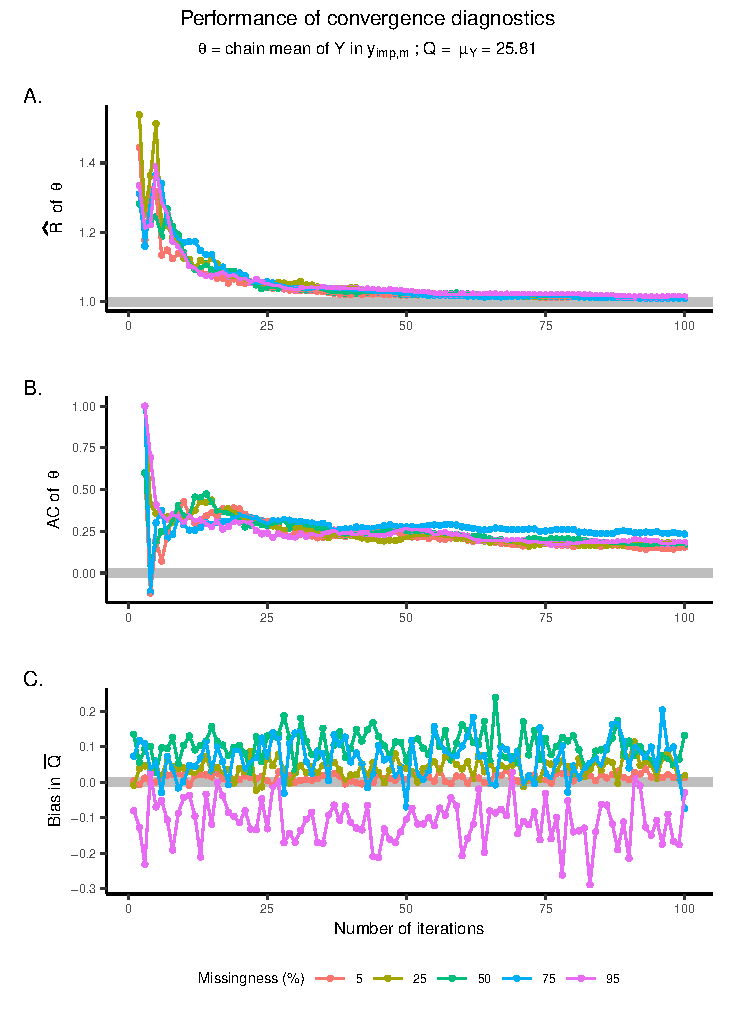
\includegraphics{manuscript_files/figure-latex/mean-1} 

}

\caption{Convergence diagnostics chain mean.}\label{fig:mean}
\end{figure}

\hypertarget{standard-deviations}{%
\subsection{Standard deviations}\label{standard-deviations}}

\textbf{Message: even with possible effect of initial values (T=1), the
algorithm is as well converged as the missingness proportion allows.}
For \(Q=\sigma_Y\) there is no effect visible of the iteration
conditions, but clearly for the p\_mis conditions. Most bias for p\_mis
= 95, followed by p\_mis=50 and 75. For the least possible bias we may
use any number of iterations \(T\geq1\), but none of the p\_mis results
in unbiased bar\{Q\}s.

There is a clear effect of the number of iterations on Rhat. Conditions
with lower Ts have more signs of non-conv, as identified by Rhat. There
is little difference between missingness conditions. Only for conditions
where \(T<5\) the missingness proportions seem to affect whether Rhat
indicates non-conv. The bias in bar\{Q\} seems unrelated to the
magnitude of Rhat. Conditions with more bias (p\_mis = 50,75,95) are not
identified to have more signs of non-convergence. The thresholds are
therefore useless (because depend mostly on t, not so much p\_mis).

AC is affected by both t and p\_mis conditions. But conditions with
worst bias (p\_mis = 50, 75, 95) are not identified as worst converging
according to AC. Moreover, only for T=3 the AC is significantly
different from zero.

\begin{figure}

{\centering 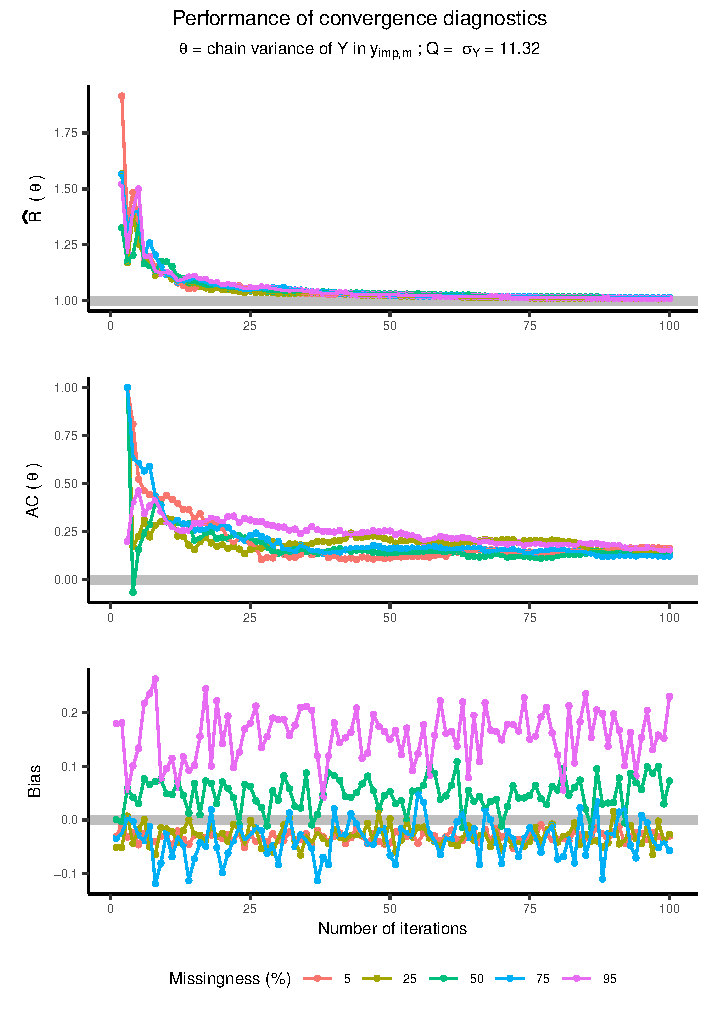
\includegraphics{manuscript_files/figure-latex/sd-1} 

}

\caption{Convergence diagnostics chain variance.}\label{fig:sd}
\end{figure}

\hypertarget{regression-coefficients}{%
\subsection{Regression coefficients}\label{regression-coefficients}}

\textbf{Message: after four iterations (T=5), the algorithm is as well
converged as the missingness proportion allows. Sooner even with lower
missingness proportions (T=1 might be ok for p\_mis=5 and 25).} The
figure for \(Q=\beta_1\) shows that the \(\bar{Q}\)s are affected by
both the number of iterations and the missingness proportion. For T=1,
the magnitude of the bias (almost) follows the order of the missingness
proportions. More missingness causes more bias in the \(\bar{Q}\). In
general, a lower nr of iterations results in more bias, but this depends
on the missingness proportion. For p\_mis=95, there is more bias in
conditions where T\textless6. When p\_mis = 50, it's T\textless3. For
p\_mis = 75 and 25, it's only for T\textless2. And conditions where
p\_mis = 5 are unaffected on average. However, none of the conditions
result in completely unbiased estimates of \(Q\).

We should see this in the conv diag: higher Rhat and AC for p\_mis=75
and 95, and for condtions where \(T<2-6\), depending on p\_mis.

Rhat depends somewhat on the missingness proportion. For conditions
where T\textless10, the Rhat values follow the p\_mis more or less. But
what we actually want to know is whether they are indicators of bias.
Conditions with the worst bias (high p\_mis, low T) have the largest
Rhat values. The thresholds are not appropriate to diagnose sufficient
convergence. All thresholds over-estimate the signs of non-convergence
compared to the bias in Qbar. However, a higher threshold than 1.2 may
result in terminating the algorithm after 3 iterations, which is
insufficient for the p\_mis = 95 condition. Threshold of 1.25 or 1.3
could work for the other p\_mis conditions.

AC is very affected by the p\_mis. The two conditions with the most bias
(p\_mis = 75 and 95) are the only ones identified as non-converging, as
they should. However, the p\_mis = 75 condition is only identified in
the T=3 condtion, while the bias is the least pronounced there. And the
AC only identifies non-convergence in the p\_mis = 95 conditions where
T\textgreater10. In the default situation, T=5, this would be
overlooked. Also, the AC shows the opposite of what you would expect
from a theta that is based on the observed data: shouldn't there be
higher autocorrelations in conditions with comparatively more observed
data in the completed datasets? I don't understand this.

\textbf{Add how interesting it is because we literally track Q and are
still not ok.}

\begin{figure}

{\centering 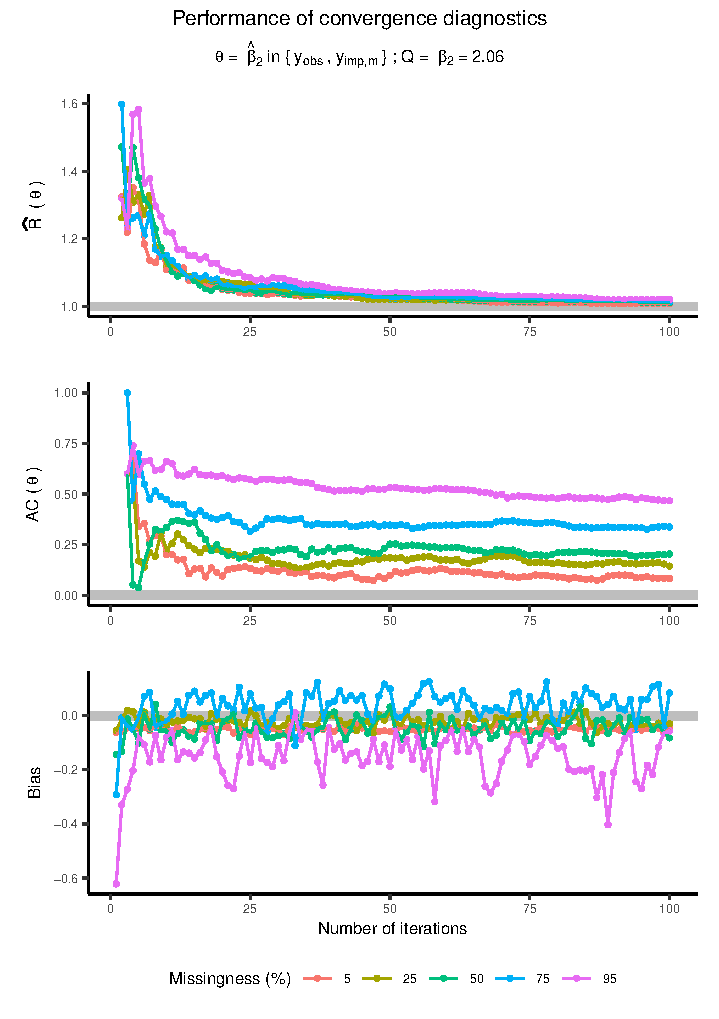
\includegraphics{manuscript_files/figure-latex/est-1} 

}

\caption{Convergence diagnostics regression coefficient.}\label{fig:est}
\end{figure}

\hypertarget{variance-explained}{%
\subsection{Variance explained}\label{variance-explained}}

\textbf{Message: after two iterations (T=3), the algorithm is as well
converged as the missingness proportion allows. Sooner even with lower
missingness proportions (T=1 might be ok for p\_mis=5 and 25).} Bias is
the worst for conditions where p\_mis = 95, T\textless3. Followed by
p\_mis = 75, T=1; and p\_mis = 50, T=1. Conditions where p\_mis = 25 or
5 seem unaffected by the number of iterations. Minimal bias is obtained
in all iteration conditions. We should see this in Rhat and AC: worst
convergence in p\_mis = 95 and 50; some non-conv in conditions where
p\_mis = 75 and T=1, and no non-conv in conditions where p\_mis = 25 or
5. The sign of the bias is logical: when there is less info in the data,
the relations between the predictors and the outcome is under-estimated.

Rhat behaves oppositely to what we wanted. The lowest Rhat values for
conditions where T\textless10 are observed for the two missingness
conditions with the worst bias. However, the highest Rhat observed is
indeed for the missingness condition with the worst bias, p\_mis =95.
But only at T=5 (while bias is no worse than anywhere else in this
p\_mis condition, conditional on iterations condition T\textgreater2).
So neither of the thresholds works perfectly.

AC shows a similar trend to the biases: more signs of non-conv for
higher p\_mis and lower T. The threshold, however, performs less well.
It identifies signs of non-convergence for all conditions where \(T=3\),
irrespective of p\_mis. Then nothing, and then for p\_mis =95,
T\textgreater7, and p\_mis=50, T \textgreater14, and p\_mis = 75,
T\textgreater20. This does not corresond to the bias in \(\bar{Q}\).
Maybe use AC\textgreater.5 at T=5 as threshold?

\begin{figure}

{\centering 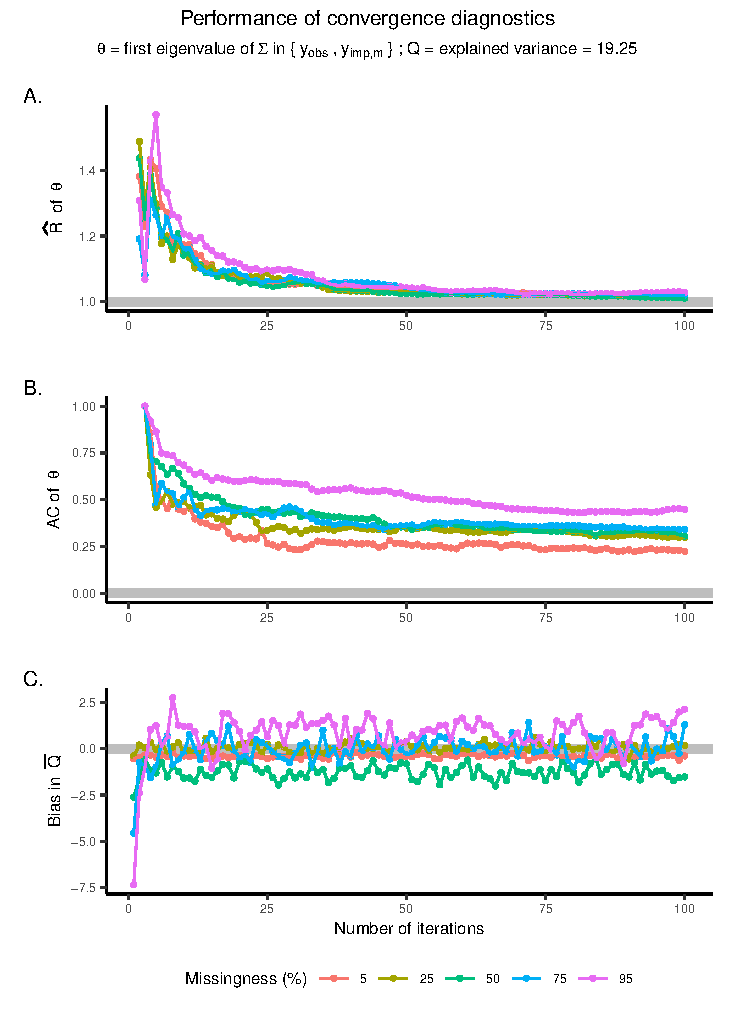
\includegraphics{manuscript_files/figure-latex/pred-1} 

}

\caption{Convergence diagnostics regression coefficient.}\label{fig:pred}
\end{figure}

\hypertarget{discussion}{%
\section{Discussion}\label{discussion}}

In short, univariate estimates seem robust against terminating the
algorithm early: There is no clear effect of the number of iterations on
the bias in these estimates. The bias in the Qs only depends on the
p\_mis. Yet, the convergence diagnostics indicate that the algorithm did
not reach a completely converged state (yet).

\(\widehat{R}\) and autocorrelation indicate that algorithmic
convergence may only be reached after twenty or even forty iterations,
while unbiased, confidence valid estimates may be obtained with as
little as one iteration. These results are in agreement with the
simulation hypothesis: \(\widehat{R}\) over-estimates the severity of
non-convergence when applied to MI procedures.

With that, we show that MICE can lead to correct outcomes when they have
not converged according to two common conv diags. This may be due to the
methods (and their thresholds) or due to the Qs (descriptives and
multivariate linear regression, not higher dimensional/more complex Qs).
More `complicated' \(Q\)s (e.g., higher-order effects or variance
components) might show bias, under- or over-coverage at higher \(T\), as
indiated by Rhat and AC. Add what \%miss has to do with it.

\hypertarget{recommendations-for-empirical-researchers}{%
\subsection{Recommendations for empirical
researchers}\label{recommendations-for-empirical-researchers}}

For empirical researchers:

\begin{enumerate}
\def\labelenumi{\arabic{enumi}.}
\item
  Check trace plots for pathological non convergence and adjust
  imputation model if necessary.
\item
  use \(\widehat{R}\) wait 1.1 ash threshold and autocorrelation with
  \textbf{?} as threshold. Keep iterating until these thresholds are
  reached.
\item
  Do not use the R function ACF. Instead, compute autocorrelations
  manually \textbf{(see e.g., {[}GitHub link{]})}.
\item
  Track your own scalar summary of interest. This is somewhat advanced
  but explained in Van Buren 2018. Compute \(\widehat{R}\) and
  autocorrelation values for this scalar summary.
\item
  \textbf{Something} about the novel \(\theta\) that is `substantive
  model-independent'.
\end{enumerate}

\hypertarget{recommendations-for-future-research}{%
\subsection{Recommendations for future
research}\label{recommendations-for-future-research}}

Further research is needed to investigate their performance under clear
violation of convergence, e.g.~dependency between predictors (predictors
with very high correlations). Also:

\begin{itemize}
\item
  Induce non-convergence with mis-specified imputation model.
\item
  More difficult missingness problems, i.e., M(N)AR instead of MCAR.
  Proper performance under a `missing completely at random' missingness
  mechanism is necessary to demonstrate the appropriateness of
  \(\widehat{R}\) and \(AC\) as non-convergence diagnostics. However,
  results may not be extrapolated to other missingness mechanisms.
\item
  Imputation technique with questionable convergence properties, e.g.,
  PMM.
\item
  Apply recommendations to empirical data and write a vignette for
  applied researchers.
\item
  Implement recommendations in ShinyMICE.
\item
  Develop an additional convergence diagnostic unique for iterative
  imputation: AC across imputations, instead of iterations.
\end{itemize}

\hypertarget{grading}{%
\section{Grading}\label{grading}}

\begin{itemize}
\item
  Scientific contribution (clear research question, convincing
  argumentation that the study adds to the scientific literature)
\item
  Theory (use of theory, clear hypotheses, relevant literature)
\item
  Method (correct data collection/handling, measures, choice and
  description of method of analysis)
\item
  Results (correct interpretation of findings, clear presentation)
\item
  Discussion and conclusions (summary, broader implications,
  limitations, future research)
\item
  Written presentation (writing, structure, tables and figures,
  references)
\end{itemize}

\bibliographystyle{sageh}
\bibliography{thesis.bib}


\end{document}
